%------------------------------------------------------------------------------
\chapter{Störkörpermessungen}
\label{sec:stoerkoerpermessung}
%------------------------------------------------------------------------------


%------------------------------------------------------------------------------
\section{Vorbereitung der Störkörpermessung}
%------------------------------------------------------------------------------

%------------------------------------------------------------------------------
\subsection{Vorbereitung des Resonators}
\label{sec:vorbereitung_resonator}
%------------------------------------------------------------------------------
Bevor mit der Störkörpermessung nach Abschnitt \ref{sec:messmethodik} begonnen werden kann, müssen noch Einstellungen am Resonator erfolgen.
Zum einen wird die Koppelschleife so gedreht, dass eine nahezu kritische Einkopplung ($\kappa \approx 1$) an die $\mathrm{TM}_{010}\text{-}\pi$-Mode des Resonators realisiert wird.
Dies kann durch eine Messung des Reflexionskoeffizienten mit dem VNA überprüft werden, da für den Fall kritischer Kopplung gemäß Gleichung \eqref{eq:resonanzkurve}
\begin{align}
	|\rho(\omega = \omega_0)| = 0
\end{align}
gilt.

Außerdem werden beide Abstimmstempel so eingestellt, dass sich eine symmetrische Feldverteilung im Resonator ausbildet.
Dazu wird die Resonanzfrequenzverschiebung durch den Störkörper in der Mitte beider Stempel-Zellen gemessen.
Ist die Frequenzverschiebung und somit auch die Amplitude elektrischen Feldes an beiden Stellen gleich, so liegt eine symmetrische Feldverteilung vor.
Anderenfalls werden die Stempel so lange gegeneinander Verfahren, bis eine Stempelstellung gefunden wurde, für die sich ein symmetrisches Feld im Resonator ausbildet.

Schließlich muss die Beschleunigungsmode auf ihre Sollfrequenz im Vakuum von $\SI{499.67}{MHz}$ durch paralleles Verfahren der Stempel abgestimmt werden.
Dabei ist zu beachten, dass die Luft im Hohlraum des Resonators zu einer zusätzlichen Verstimmung führt.
Ist der Resonator durch ein Medium der relativen Permittivität~$\varepsilon_\mathrm{r}$ und Permeabilität~$\mu_\mathrm{r}$ ausgefüllt, so kann die Verstimmung der Resonanzfrequenzen durch
\begin{align}
	\nu_0^\mathrm{Med} = \frac{\nu_0^\mathrm{Vak}}{\sqrt{\varepsilon_\mathrm{r} \mu_\mathrm{r}}}
	\label{eq:resonanzfrequenz_medium}
\end{align}
beschrieben werden \cite{pusch}.
Mit der relativen Permittivität trockener Luft~$\varepsilon_\mathrm{r}^\mathrm{Luft} = \num{1.0005364}$ unter Normalbedingungen \cite{CRC}, vernachlässigbarer relativer Permeabilität~($\mu_\mathrm{r} \approx 1$) und der Sollfrequenz im Vakuum~$\nu_0^\mathrm{Vak}$ folgt die Frequenz der Beschleunigungsmode
\begin{align}
	\nu_0^\mathrm{Luft} = \SI{499.54}{MHz}
\end{align}
für den luftgefüllten Resonator.
Da diese Frequenz mit Temperatur und Luftfeuchtigkeit variiert, ist ein exaktes Abstimmen auf diese Frequenz nicht zweckmäßig und es genügt die grobe Einstellung mit einer Genauigkeit von einigen \si{\kilo\hertz}.

%------------------------------------------------------------------------------
\subsection{Bestimmung der Störkörperkonstante}
%------------------------------------------------------------------------------

Zur Berechnung der Störkörperkonstante~$\alpha_\mathrm{s}$ des kugelförmigen Störkörpers aus PTFE mit einem Durchmesser $D = \SI{20.05 +- 0.05}{mm}$ und der zentrischen Bohrung mit dem Durchmesser~\mbox{$d = \SI{1.3 +- 0.05}{mm}$} kann Gleichung \eqref{eq:stoerkoerperkonstante} verwendet werden.
Die relative Permittivität von PTFE beträgt im Mittel $\varepsilon_\mathrm{r} = \num{2.1}$ und variiert mit der Dichte und Kristallinität des Materials \cite{CRC}.
Daher wird für den verwendeten Störkörper $\varepsilon_\mathrm{r} = \num{2.1 +- 0.05}$ angenommen.
Es folgt für die Störkörperkonstante
\begin{align}
	\alpha_\mathrm{s} = \SI{2.99 +- 0.11e-17}{\ampere\second\metre\squared\per\volt} \eqcomma
	\label{eq:stoerkoerperkonstante_ptfe}
\end{align}
wobei das fehlende Volumen der zentrischen Bohrung beachtet wurde.

Bei der Bestimmung der elektrischen Felder gemäß Gleichung \eqref{eq:skm_e_feld_normiert}, wirkt der Fehler der Störkörperkonstanten systematisch auf das resultierende Feld.
Dieser systematische Einfluss muss insbesondere bei der Integration des Feldes über die Störkörperposition (Bestimmung von Beschleunigungsspannung und Shuntimpedanz) gesondert betrachtet werden.
Um diesen Fehler zu verringern, könnte eine direkte Bestimmung der Störkörperkonstanten in einem Referenzresonator durchgeführt werden.
Darauf wurde jedoch in dieser Arbeit verzichtet, da mit einem relativen Fehler von unter $\SI{4}{\percent}$ eine ausreichende Genauigkeit vorliegt.

%------------------------------------------------------------------------------
\subsection{Bestimmung von Resonanzfrequenz und Güte}
\label{sec:resfreq_guete}
%------------------------------------------------------------------------------
Die Bestimmung von Resonanzfrequenz und Güte der Resonatormoden kann anhand des gemessenen Reflexionsspektrums der jeweiligen Resonanz erfolgen.
Dazu wird eine Kurve gemäß Gleichung \eqref{eq:resonanzkurve} nach der Methode der kleinsten Quadrate an das gemessene Spektrum angepasst.
Dies wird, am Beispiel der $\mathrm{TM}_{010}\text{-}\pi$-Beschleunigungsmode von PETRA-III, in Abbildung \ref{fig:guetefit} dargestellt.
\begin{figure}[htb]
  \centering
  % GNUPLOT: LaTeX picture with Postscript
\begingroup
  \makeatletter
  \providecommand\color[2][]{%
    \GenericError{(gnuplot) \space\space\space\@spaces}{%
      Package color not loaded in conjunction with
      terminal option `colourtext'%
    }{See the gnuplot documentation for explanation.%
    }{Either use 'blacktext' in gnuplot or load the package
      color.sty in LaTeX.}%
    \renewcommand\color[2][]{}%
  }%
  \providecommand\includegraphics[2][]{%
    \GenericError{(gnuplot) \space\space\space\@spaces}{%
      Package graphicx or graphics not loaded%
    }{See the gnuplot documentation for explanation.%
    }{The gnuplot epslatex terminal needs graphicx.sty or graphics.sty.}%
    \renewcommand\includegraphics[2][]{}%
  }%
  \providecommand\rotatebox[2]{#2}%
  \@ifundefined{ifGPcolor}{%
    \newif\ifGPcolor
    \GPcolortrue
  }{}%
  \@ifundefined{ifGPblacktext}{%
    \newif\ifGPblacktext
    \GPblacktexttrue
  }{}%
  % define a \g@addto@macro without @ in the name:
  \let\gplgaddtomacro\g@addto@macro
  % define empty templates for all commands taking text:
  \gdef\gplbacktext{}%
  \gdef\gplfronttext{}%
  \makeatother
  \ifGPblacktext
    % no textcolor at all
    \def\colorrgb#1{}%
    \def\colorgray#1{}%
  \else
    % gray or color?
    \ifGPcolor
      \def\colorrgb#1{\color[rgb]{#1}}%
      \def\colorgray#1{\color[gray]{#1}}%
      \expandafter\def\csname LTw\endcsname{\color{white}}%
      \expandafter\def\csname LTb\endcsname{\color{black}}%
      \expandafter\def\csname LTa\endcsname{\color{black}}%
      \expandafter\def\csname LT0\endcsname{\color[rgb]{1,0,0}}%
      \expandafter\def\csname LT1\endcsname{\color[rgb]{0,1,0}}%
      \expandafter\def\csname LT2\endcsname{\color[rgb]{0,0,1}}%
      \expandafter\def\csname LT3\endcsname{\color[rgb]{1,0,1}}%
      \expandafter\def\csname LT4\endcsname{\color[rgb]{0,1,1}}%
      \expandafter\def\csname LT5\endcsname{\color[rgb]{1,1,0}}%
      \expandafter\def\csname LT6\endcsname{\color[rgb]{0,0,0}}%
      \expandafter\def\csname LT7\endcsname{\color[rgb]{1,0.3,0}}%
      \expandafter\def\csname LT8\endcsname{\color[rgb]{0.5,0.5,0.5}}%
    \else
      % gray
      \def\colorrgb#1{\color{black}}%
      \def\colorgray#1{\color[gray]{#1}}%
      \expandafter\def\csname LTw\endcsname{\color{white}}%
      \expandafter\def\csname LTb\endcsname{\color{black}}%
      \expandafter\def\csname LTa\endcsname{\color{black}}%
      \expandafter\def\csname LT0\endcsname{\color{black}}%
      \expandafter\def\csname LT1\endcsname{\color{black}}%
      \expandafter\def\csname LT2\endcsname{\color{black}}%
      \expandafter\def\csname LT3\endcsname{\color{black}}%
      \expandafter\def\csname LT4\endcsname{\color{black}}%
      \expandafter\def\csname LT5\endcsname{\color{black}}%
      \expandafter\def\csname LT6\endcsname{\color{black}}%
      \expandafter\def\csname LT7\endcsname{\color{black}}%
      \expandafter\def\csname LT8\endcsname{\color{black}}%
    \fi
  \fi
    \setlength{\unitlength}{0.0500bp}%
    \ifx\gptboxheight\undefined%
      \newlength{\gptboxheight}%
      \newlength{\gptboxwidth}%
      \newsavebox{\gptboxtext}%
    \fi%
    \setlength{\fboxrule}{0.5pt}%
    \setlength{\fboxsep}{1pt}%
\begin{picture}(6802.00,4534.00)%
    \gplgaddtomacro\gplbacktext{%
      \csname LTb\endcsname%
      \put(814,704){\makebox(0,0)[r]{\strut{}0{,}0}}%
      \csname LTb\endcsname%
      \put(814,1417){\makebox(0,0)[r]{\strut{}0{,}2}}%
      \csname LTb\endcsname%
      \put(814,2130){\makebox(0,0)[r]{\strut{}0{,}4}}%
      \csname LTb\endcsname%
      \put(814,2843){\makebox(0,0)[r]{\strut{}0{,}6}}%
      \csname LTb\endcsname%
      \put(814,3556){\makebox(0,0)[r]{\strut{}0{,}8}}%
      \csname LTb\endcsname%
      \put(814,4269){\makebox(0,0)[r]{\strut{}1{,}0}}%
      \csname LTb\endcsname%
      \put(1835,484){\makebox(0,0){\strut{}499{,}48}}%
      \csname LTb\endcsname%
      \put(3200,484){\makebox(0,0){\strut{}499{,}50}}%
      \csname LTb\endcsname%
      \put(4565,484){\makebox(0,0){\strut{}499{,}52}}%
      \csname LTb\endcsname%
      \put(5930,484){\makebox(0,0){\strut{}499{,}54}}%
    }%
    \gplgaddtomacro\gplfronttext{%
      \csname LTb\endcsname%
      \put(176,2486){\rotatebox{-270}{\makebox(0,0){\strut{}Reflektionskoeffizient $|\rho|$}}}%
      \put(3675,154){\makebox(0,0){\strut{}Frequenz $\nu$ / \si{MHz}}}%
      \csname LTb\endcsname%
      \put(5418,1097){\makebox(0,0)[r]{\strut{}Messpunkte}}%
      \csname LTb\endcsname%
      \put(5418,877){\makebox(0,0)[r]{\strut{}Anpassung}}%
    }%
    \gplbacktext
    \put(0,0){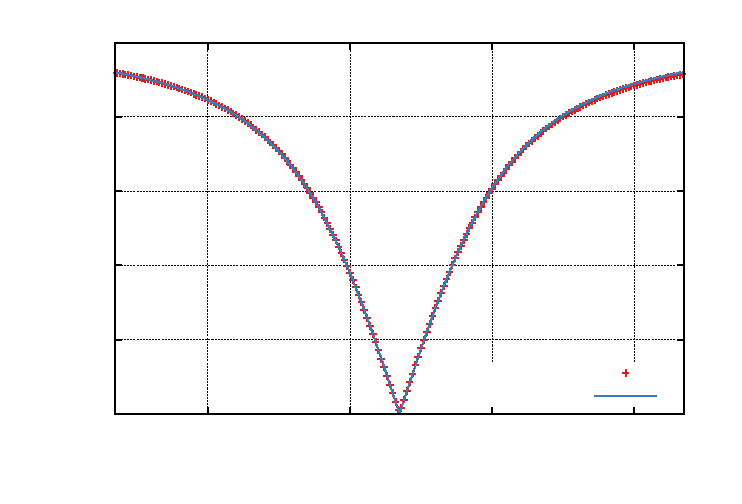
\includegraphics{./plots/guete_fit_pi}}%
    \gplfronttext
  \end{picture}%
\endgroup

  \caption[Anpassung der Resonanzkurve an das Reflexionsspektrum der $\mathrm{TM}_{010}~\pi$-Mode von PETRA-III]{Anpassung der Resonanzkurve~\eqref{eq:resonanzkurve} an ein gemessenes Reflexionsspektrum der $\mathrm{TM}_{010}\text{-}\pi$-Mode von PETRA-III. Aus Gründen der Übersicht wurde nur jeder 10.\ Messpunkt des VNA aufgetragen. Die Anpassung liefert die Resonanzfrequenz~$\nu_0 = \SI{499.537}{MHz}$ (Anpassungsfehler vernachlässigbar), Güte~$Q_0 = \num{29560 +- 20}$ und den Koppelfaktor~$\kappa = \num{1.013 +- 0.001}$.}
  \label{fig:guetefit}
\end{figure}
Um eine bessere Abschätzung der Fehler zu erlauben, wurden zu jeder Resonatormode mehrere Reflexionsspektren aufgenommen und an jedes Spektrum eine Anpassung durchgeführt.
Die resultierenden Ergebnisse folgen aus der Bildung des Mittelwerts der angepassten Parameter.
Da die Resonanzfrequenz der Moden mit der Temperatur der Kavität schwankt, wird auf eine Angabe des Fehlers verzichtet.
Darüber hinaus kann der Einfluss von dielektrischen Verlusten der Luft auf die Güte des Resonators vernachlässigt werden \cite{pozar}.

%------------------------------------------------------------------------------
\section{Vermessung der $\mathrm{TM}_{010}$-Resonatormoden}
\label{sec:tm010_messung}
%------------------------------------------------------------------------------
Die folgenden Abschnitte widmen sich der Auswertung der Störkörpermessungen an den $\mathrm{TM}_{010}$-Resonatormoden von PETRA-III und PETRA-IV, welche gemäß Abschnitt \ref{sec:messmethodik} durchgeführt wurden.
Für beide Resonatoren wurden die $\pi,\, 2/3~\pi, \, 1/3~\pi$ und $0$-Moden vermessen.
Die restlichen Moden der siebenzelligen Resonatorkette, die nach den Erläuterungen in Abschnitt \ref{sec:petra_resonator} erwartet werden, konnten nicht vermessen werden.
Dies ist der Fall, da diese Moden ein verschwindendes elektrisches und magnetisches Feld in der mittleren Zelle des Resonators aufweisen (vgl.\ Abb.\ \ref{fig:spektrum_tm010} f.) und daher nicht oder nur schwach über die Koppelschleife angeregt werden können.

Beide Resonatoren wurden mit einer Schrittweite des Störkörpers von \SI{5}{mm} vermessen, was \num{60} Messpunkten pro Zelle entspricht.
Dadurch sind die gemessenen Feldverteilungen durch das Ortsauflösungsvermögen des verwendeten Störkörpers begrenzt.

\subsection{Auswertung der Messdaten}
Nachdem die Güte~$Q_0$, Resonanzfrequenz~$\nu_0$ und Störkörperkonstante~$\alpha_\mathrm{s}$ bestimmt wurde, kann die Amplitude des elektrischen Feldes (normiert auf die Wurzel der Verlustleistung $P_\mathrm{V}$) gemäß Gleichung \eqref{eq:skm_e_feld_normiert} berechnet werden.
Außerdem kann das effektive elektrische Feld, das ein ultrarelativistisches Teilchen erfährt, welches den Resonator passiert, berechnet und somit der Laufzeitfaktor~$\Lambda$ aus Gleichung \eqref{eq:laufzeitfaktor} bestimmt werden.
Dazu muss neben der harmonischen Zeitabhängigkeit auch die Phasenbeziehung (vgl.\ Abb.\ \ref{fig:phasenbeziehung}) zwischen den einzelnen Zellen beachtet werden.
Darüber hinaus wird die Eintrittsphase des Teilchens in den Resonator so gewählt, dass der Laufzeitfaktor~$\Lambda$ bzw.\ die effektive Shuntimpedanz~$R_\mathrm{S}^\mathrm{eff}$ maximiert wird.

Dies wurde am Beispiel der $\pi$-Mode des PETRA-III Resonators in Abbildung \ref{fig:bsp_feld_tm010pi_petra3} dargestellt.
Im Anhang \ref{app:tm010_felder} wurden die Felder aller vermessenen $\mathrm{TM}_{010}$-Resonatormoden beider Resonatoren zusammengestellt.  
\begin{figure}[h]
	\centering
	% GNUPLOT: LaTeX picture with Postscript
\begingroup
  \makeatletter
  \providecommand\color[2][]{%
    \GenericError{(gnuplot) \space\space\space\@spaces}{%
      Package color not loaded in conjunction with
      terminal option `colourtext'%
    }{See the gnuplot documentation for explanation.%
    }{Either use 'blacktext' in gnuplot or load the package
      color.sty in LaTeX.}%
    \renewcommand\color[2][]{}%
  }%
  \providecommand\includegraphics[2][]{%
    \GenericError{(gnuplot) \space\space\space\@spaces}{%
      Package graphicx or graphics not loaded%
    }{See the gnuplot documentation for explanation.%
    }{The gnuplot epslatex terminal needs graphicx.sty or graphics.sty.}%
    \renewcommand\includegraphics[2][]{}%
  }%
  \providecommand\rotatebox[2]{#2}%
  \@ifundefined{ifGPcolor}{%
    \newif\ifGPcolor
    \GPcolortrue
  }{}%
  \@ifundefined{ifGPblacktext}{%
    \newif\ifGPblacktext
    \GPblacktexttrue
  }{}%
  % define a \g@addto@macro without @ in the name:
  \let\gplgaddtomacro\g@addto@macro
  % define empty templates for all commands taking text:
  \gdef\gplbacktext{}%
  \gdef\gplfronttext{}%
  \makeatother
  \ifGPblacktext
    % no textcolor at all
    \def\colorrgb#1{}%
    \def\colorgray#1{}%
  \else
    % gray or color?
    \ifGPcolor
      \def\colorrgb#1{\color[rgb]{#1}}%
      \def\colorgray#1{\color[gray]{#1}}%
      \expandafter\def\csname LTw\endcsname{\color{white}}%
      \expandafter\def\csname LTb\endcsname{\color{black}}%
      \expandafter\def\csname LTa\endcsname{\color{black}}%
      \expandafter\def\csname LT0\endcsname{\color[rgb]{1,0,0}}%
      \expandafter\def\csname LT1\endcsname{\color[rgb]{0,1,0}}%
      \expandafter\def\csname LT2\endcsname{\color[rgb]{0,0,1}}%
      \expandafter\def\csname LT3\endcsname{\color[rgb]{1,0,1}}%
      \expandafter\def\csname LT4\endcsname{\color[rgb]{0,1,1}}%
      \expandafter\def\csname LT5\endcsname{\color[rgb]{1,1,0}}%
      \expandafter\def\csname LT6\endcsname{\color[rgb]{0,0,0}}%
      \expandafter\def\csname LT7\endcsname{\color[rgb]{1,0.3,0}}%
      \expandafter\def\csname LT8\endcsname{\color[rgb]{0.5,0.5,0.5}}%
    \else
      % gray
      \def\colorrgb#1{\color{black}}%
      \def\colorgray#1{\color[gray]{#1}}%
      \expandafter\def\csname LTw\endcsname{\color{white}}%
      \expandafter\def\csname LTb\endcsname{\color{black}}%
      \expandafter\def\csname LTa\endcsname{\color{black}}%
      \expandafter\def\csname LT0\endcsname{\color{black}}%
      \expandafter\def\csname LT1\endcsname{\color{black}}%
      \expandafter\def\csname LT2\endcsname{\color{black}}%
      \expandafter\def\csname LT3\endcsname{\color{black}}%
      \expandafter\def\csname LT4\endcsname{\color{black}}%
      \expandafter\def\csname LT5\endcsname{\color{black}}%
      \expandafter\def\csname LT6\endcsname{\color{black}}%
      \expandafter\def\csname LT7\endcsname{\color{black}}%
      \expandafter\def\csname LT8\endcsname{\color{black}}%
    \fi
  \fi
    \setlength{\unitlength}{0.0500bp}%
    \ifx\gptboxheight\undefined%
      \newlength{\gptboxheight}%
      \newlength{\gptboxwidth}%
      \newsavebox{\gptboxtext}%
    \fi%
    \setlength{\fboxrule}{0.5pt}%
    \setlength{\fboxsep}{1pt}%
\begin{picture}(8502.00,5668.00)%
    \gplgaddtomacro\gplbacktext{%
      \csname LTb\endcsname%
      \put(1078,704){\makebox(0,0)[r]{\strut{}-1000}}%
      \csname LTb\endcsname%
      \put(1078,1291){\makebox(0,0)[r]{\strut{}0}}%
      \csname LTb\endcsname%
      \put(1078,1879){\makebox(0,0)[r]{\strut{}1000}}%
      \csname LTb\endcsname%
      \put(1078,2466){\makebox(0,0)[r]{\strut{}2000}}%
      \csname LTb\endcsname%
      \put(1078,3054){\makebox(0,0)[r]{\strut{}3000}}%
      \csname LTb\endcsname%
      \put(1078,3641){\makebox(0,0)[r]{\strut{}4000}}%
      \csname LTb\endcsname%
      \put(1078,4228){\makebox(0,0)[r]{\strut{}5000}}%
      \csname LTb\endcsname%
      \put(1078,4816){\makebox(0,0)[r]{\strut{}6000}}%
      \csname LTb\endcsname%
      \put(1078,5403){\makebox(0,0)[r]{\strut{}7000}}%
      \csname LTb\endcsname%
      \put(1210,484){\makebox(0,0){\strut{}0}}%
      \csname LTb\endcsname%
      \put(2763,484){\makebox(0,0){\strut{}500}}%
      \csname LTb\endcsname%
      \put(4316,484){\makebox(0,0){\strut{}1000}}%
      \csname LTb\endcsname%
      \put(5869,484){\makebox(0,0){\strut{}1500}}%
      \csname LTb\endcsname%
      \put(7422,484){\makebox(0,0){\strut{}2000}}%
    }%
    \gplgaddtomacro\gplfronttext{%
      \csname LTb\endcsname%
      \put(176,3053){\rotatebox{-270}{\makebox(0,0){\strut{}$\frac{E_0(z)}{\sqrt{P_\mathrm{V}}}$ / \si{\volt\per\metre\per\watt\tothe{0{,}5}}}}}%
      \put(4657,154){\makebox(0,0){\strut{}$z$ / \si{mm}}}%
      \csname LTb\endcsname%
      \put(7382,5230){\makebox(0,0)[r]{\strut{}Amplitude}}%
      \csname LTb\endcsname%
      \put(7382,5010){\makebox(0,0)[r]{\strut{}effektives Feld}}%
    }%
    \gplbacktext
    \put(0,0){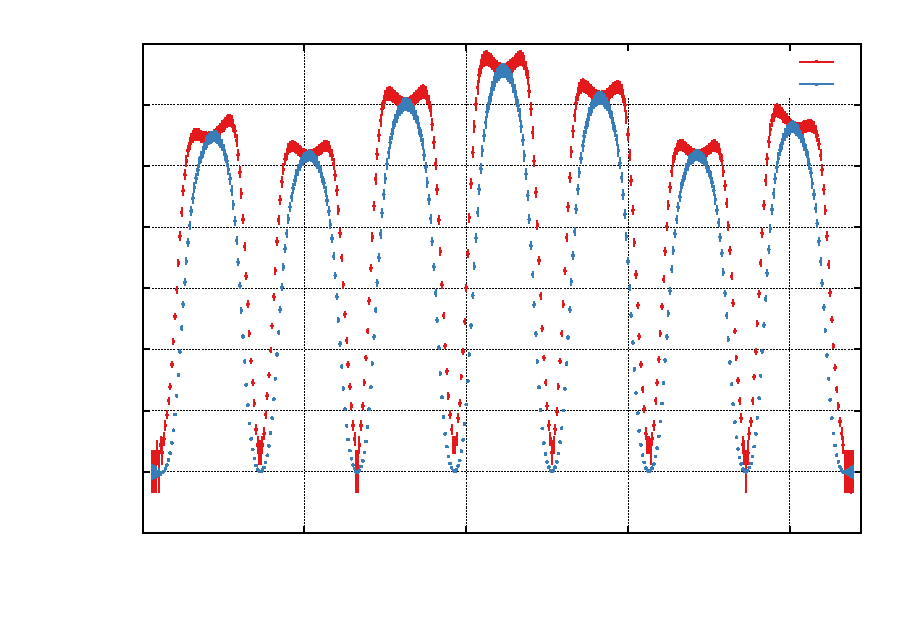
\includegraphics{./plots/PETRA-IV/pi}}%
    \gplfronttext
  \end{picture}%
\endgroup

	\caption[Elektrische Feldverteilung der $\mathrm{TM}_{010}\text{-}\pi$-Beschleunigungsmode von PETRA-III]{Elektrische Feldverteilung der $\mathrm{TM}_{010}\text{-}\pi$-Beschleunigungsmode von PETRA-III. Die Position~$z$ ist relativ zum Vakuumflansch angegeben.}
	\label{fig:bsp_feld_tm010pi_petra3}
\end{figure}

Schließlich können die charakteristischen Größen der $\mathrm{TM}_{010}$-Moden bestimmt werden, wobei die folgenden Überlegungen auf dem Inhalt von Abschnitt \ref{sec:resonator_charakteristiken} basieren.
Zunächst erfolgt die Berechnung der longitudinalen Shuntimpedanzen~$R_\mathrm{S}$, indem Gleichung \eqref{eq:beschleunigungsspannung} in \eqref{eq:shuntimpedanz} eingesetzt wird, sodass man
\begin{align}
	R_\mathrm{S} = \frac{1}{2} \left( \int_0^L \frac{|\ve_0(z)|}{\sqrt{P_\mathrm{V}}} \, \mathrm{d}z \right)^2
\end{align}
erhält.
Demnach kann die Shuntimpedanz durch Integration der (normierten) elektrischen Feldamplitude über die Länge~$L$ des Resonators gewonnen werden.
Diese Integration sowie die hierauf folgenden Integrationen erfolgen dabei numerisch durch die Trapezregel.
Ebenso kann der Laufzeitfaktor~$\Lambda$ als das Verhältnis des Integrals von effektivem Feld zum Integral der Feldamplitude berechnet werden.
Dieser dient der Berechnung der effektiven Shuntimpedanz~$R_\mathrm{S}^\mathrm{eff}$, die nun durch Gleichung \eqref{eq:eff_shuntimpedanz} bestimmt werden kann.
Alternativ kann die effektive Shuntimpedanz durch Integration über das effektive Feld, analog zur Berechnung der Shuntimpedanz, ermittelt werden.

Die Kenngrößen der verschiedenen $\mathrm{TM}_{010}$-Resonatormoden und deren longitudinalen Shuntimpedanzen wurden in Tabelle \ref{tab:shuntimpedanzen_tm010} zusammengestellt.
\begin{table}[htb]
	\begin{subtable}{1\textwidth}
		\centering
		\begin{tabular}{
		c
		S[table-format=3.2]
		S[table-format=5.0(3), table-align-uncertainty = true]
		S[table-format=2.1(3), table-align-uncertainty = true]
		S[table-format=0.3(1), table-align-uncertainty = true]
		S[table-format=3.2(2)e1, table-align-uncertainty = true]
		}
	\toprule
	{$\Delta \varphi$} & {$\nu_0$ / \si{MHz}} & {$Q_0$} & {$R_\mathrm{S}$ / \si{\mega\ohm}} & {$\Lambda$} & {$R_\mathrm{S}^\mathrm{eff}$ / \si{\ohm}} \\
	\midrule
	$\pi$ & 499.67 & 29556+-110 & 43.6+-1.6 & 0.767+-0.002 & 25.65+-0.91e6 \\[0.25em]
	$\frac{2}{3}\pi$ & 501.14 & 31741+-86 & 37.8+-1.4 & 0.092+-0.002 & 320+-11e3 \\[0.25em]
	$\frac{1}{3}\pi$ & 505.37 & 32707+-118 & 42.3+-1.5 & 0.141+-0.001 & 842+-30e3 \\[0.25em]
	$0$ & 508.61 & 35999+-66 & 46.2+-1.7 & 0.010+-0.001 & 5.0+-0.5e3 \\
	\bottomrule
\end{tabular}

		\caption{PETRA-III}
	\end{subtable}
	\begin{subtable}{1\textwidth}
		\centering
		\begin{tabular}{
		c
		S[table-format=3.2]
		S[table-format=5.0(3), table-align-uncertainty = true]
		S[table-format=2.1(3), table-align-uncertainty = true]
		S[table-format=0.3(1), table-align-uncertainty = true]
		p{-1mm}
		S[table-format=2.2]
		@{ $\pm$ }
		S[table-format= 1.2]
		@{\,) $\cdot$ }
		l
		}
	\toprule
	{$\Delta \varphi$} & {$\nu_0$ / \si{MHz}} & {$Q_0$} & {$R_\mathrm{S}$ / \si{\mega\ohm}} & {$\Lambda$} & \multicolumn{4}{c}{$R_\mathrm{S}^\mathrm{eff}$ / \si{\ohm}} \\
	\midrule
	$\pi$ & 499.67 & 28200+-176 & 41.6+-1.5 & 0.767+-0.001 & ( & 24.47 & 0.87 & $10^6$ \\[0.25em]
	$\frac{2}{3}\pi$ & 501.17 & 31356+-218 & 37.5+-1.4 & 0.056+-0.001 & ( & 115.3 & 4.1 & $10^3$ \\[0.25em]
	$\frac{1}{3}\pi$ & 505.43 & 32732+-54 & 42.3+-1.5 & 0.041+-0.001 & ( & 69.8 & 2.4 & $10^3$ \\[0.25em]
	$0$ & 508.61 & 35445+-59 & 45.4+-1.6 & 0.013+-0.001 & ( & 7.7 & 0.6 & $10^3$ \\
	\bottomrule
\end{tabular}

		\caption{PETRA-IV}
	\end{subtable}
	\caption[Longitudinale Shuntimpedanzen der $\mathrm{TM}_{010}$-Moden von PETRA-III und PETRA-IV]{Longitudinale Shuntimpedanzen der vermessenen $\mathrm{TM}_{010}$-Moden beider PETRA-Resonatoren. Die Resonanzfrequenz~$\nu_0$ wurde gemäß Abschnitt \ref{sec:vorbereitung_resonator} auf die Frequenz des evakuierten Resonators umgerechnet.}
	\label{tab:shuntimpedanzen_tm010}
\end{table}

\subsection{Vergleich und Interpretation der Ergebnisse}
Wie zu erwarten, zeigt die $\pi$-Mode beider Resonatoren mit einem Laufzeitfaktor von \SI{76,7}{\percent} die höchste effektive Shuntimpedanz.
Dies ist der Fall, da ein ultrarelativistisches Teilchen zum Durchqueren einer Zelle der Länge \SI{30}{\centi\metre} bei einer treibenden Hochfrequenz von \SI{499.67}{MHz} genau eine halbe Periode der Hochfrequenz benötigt.
Durch den Phasensprung von $\pi$ zwischen jeder Zelle bedeutet dies, dass das Teilchen stets ein elektrisches Feld erfährt, welches in dessen Bewegungsrichtung zeigt (vgl.\ Abschnitt \ref{app:tm010_felder}).
Im Vergleich dazu sind die restlichen $\mathrm{TM}_{010}$-Moden mit effektiven Shuntimpedanzen der Größenordnung von einigen \si{\kilo\ohm} ungeeignet für die effiziente Beschleunigung geladener Teilchen.
Dahingehend soll sich die Diskussion auf die $\pi$-Beschleunigungsmode beschränken.

Laut Herstellerangaben liegt die Güte der siebenzelligen PETRA-Resonatoren im Bereich von \num{29000} bis \num{36000} bei einem Nominalwert von \num{32800} \cite{desy_petra}.
PETRA-IV unterschreitet somit die Untergrenze der Güte um etwa \num{800} und lediglich PETRA-III fällt in den angegebenen Bereich.
Außerdem unterschreiten beide deutlich die nominale Güte, was möglicherweise darauf zurückzuführen ist, dass beide Resonatoren über längere Zeit belüftet waren und so eine Oxidation der Kupferoberfläche stattgefunden hat, die eine Vergrößerung der Verluste des Resonators zur Folge hat.
Im Folgenden wird diese Abweichung auch bei den Shuntimpedanzen auftreten, da diese eine lineare Abhängigkeit von der Güte der Resonatormode aufweist.

Der Hersteller gibt eine nominale (effektive) Shuntimpedanz von \SI{28.1}{\mega\ohm} an \cite{desy_petra}, welche gemäß der vorigen Erläuterungen nicht erreicht werden kann.
Ein Vergleich ist dennoch möglich, wenn der Geometriefaktor $R_\mathrm{S}^\mathrm{eff} / Q_0$ der Beschleunigungsmode betrachtet wird.
Für beide Resonatoren erhält man den Geometriefaktor der $\pi$-Mode von
\begin{align}
	\frac{R_\mathrm{S}^\mathrm{eff}}{Q_0} = \SI{868+-32}{\ohm} \eqcomma
\end{align}
welcher unabhängig von der Verlustleistung des jeweiligen Resonators ist.
Gemäß der Simulation der Kavität durch den Hersteller mit MAFIA\texttrademark\footnote{Programm zur numerischen Simulation elektromagnetischer Felder und Vorgänger des \textit{CST Microwave Studio\textsuperscript{\textregistered}}.} beträgt der Geometriefaktor \SI{856}{\ohm} \cite{desy_petra} und steht somit in guter Übereinstimmung mit den gemessenen Werten.

Wird eine treibende Hochfrequenzleistung~$P_\mathrm{HF}$ bei kritischer Kopplung (die Verlustleistung~$P_\mathrm{V}$ entspricht dann $P_\mathrm{HF}$) des Resonators angenommen, so erhält man die effektive Beschleunigungsspannung gemäß Gleichung \eqref{eq:eff_shuntimpedanz}
\begin{align}
	U_\mathrm{eff} = \sqrt{2 R_\mathrm{S}^\mathrm{eff} P_\mathrm{HF}} \eqdot
\end{align}
Wird beispielsweise zum Betrieb der Resonatoren ein $\SI{200}{\kilo\watt}$-Klystron genutzt, dessen Leistung durch ein magisches T (Leistungsteiler auf Hohlleiterbasis) gleichmäßig auf beide Resonatoren aufgeteilt wird, so erhält man effektive Beschleunigungsspannungen von
\begin{align}
	U_\mathrm{eff}^\mathrm{P-III} = \SI{2.265 +- 0.041}{\mega\volt} \qquad \text{und} \qquad U_\mathrm{eff}^\mathrm{P-IV} = \SI{2.212 +- 0.040}{\mega\volt} 
\end{align}
unter der Verwendung der gemessenen Shuntimpedanzen.
Der Vergleich mit den aktuell in \mbox{ELSA} verbauten fünfzelligen Resonatoren vom Typ PETRA mit einer effektiven Shuntimpedanz von \SI{15}{\mega\ohm} liefert bei gleicher eingekoppelter Leistung eine effektive Beschleunigungsspannung $U_\mathrm{eff} = \SI{1.73}{\mega\volt}$.
Dies zeigt eine wesentlich effizientere Beschleunigung in den siebenzelligen Resonatoren gegenüber den fünfzelligen und ist der Hauptgrund für die Konstruktion mehrzelliger Beschleunigungsresonatoren.

\section{Vermessung von Moden höherer Ordnung}
\label{sec:hom_messung}
Schließlich wurde eine Vermessung von Moden höherer Ordnung von PETRA-III durchgeführt.
Eine Vorauswahl der zu vermessenen Moden wurde dabei anhand deren Güte getroffen, so dass nur Resonanzen mit Güten der Größenordnung $10^4$ und größer in Betrachtung gezogen wurden.
Außerdem wurde ein Schwerpunkt auf die $\mathrm{TM}_{021}$-Mode bei ca. \SI{1.46}{GHz} gesetzt, da diese gemäß \cite{schedler} eine effektive Shuntimpedanz in der Größenordnung der Fundamentalmode besitzt.
Die Vermessung und Teile der Auswertung dieser Moden erfolgt analog zu Abschnitt~\ref{sec:tm010_messung} und soll daher nicht wiederholt werden.
Die Abweichungen werden im folgenden Abschnitt dargestellt.

\subsection{Auswertung der Messdaten}
Zur Auswertung der vermessenen Feldverteilungen muss zunächst die Phasenbeziehung der Felder in den einzelnen Zellen bestimmt werden.
Dazu werden Simulationen der Eigenmoden eines vereinfachten Modells des siebenzelligen PETRA-Resonators von \cite{schedler_pm} mit \textit{CST Microwave Studio\textsuperscript{\textregistered}} (CST-MWS) durchgeführt.
Aufgrund der Tatsache, dass ein vereinfachtes Modell der Kavität genutzt wird, kommt es teilweise zu großen Abweichungen der Resonanzfrequenz zwischen Simulation und Messung.
Darüber hinaus treten Diskrepanzen zwischen simulierten und gemessenen Feldamplituden auf.
Diese Abweichungen sind unter anderem auf die rudimentäre Modellierung der Nasenkegel und Abstimmstempel zurückzuführen.
Außerdem ist die Zelle der Einkopplung ohne Koppelschleife modelliert.
Dennoch ist eine Identifizierung der meisten vermessenen Resonatormoden anhand charakteristischer Merkmale der Feldverteilung zu vollziehen.
In Abbildung~\ref{fig:cst_sim_tm111} wurden exemplarisch die (qualitativen) Ergebnisse einer Simulation der vermessenen $\mathrm{TM}_{111}$-Mode durch CST-MWS gezeigt. 
\begin{figure}[h]
	\centering
	\begin{subfigure}{1\textwidth}
		\centering
		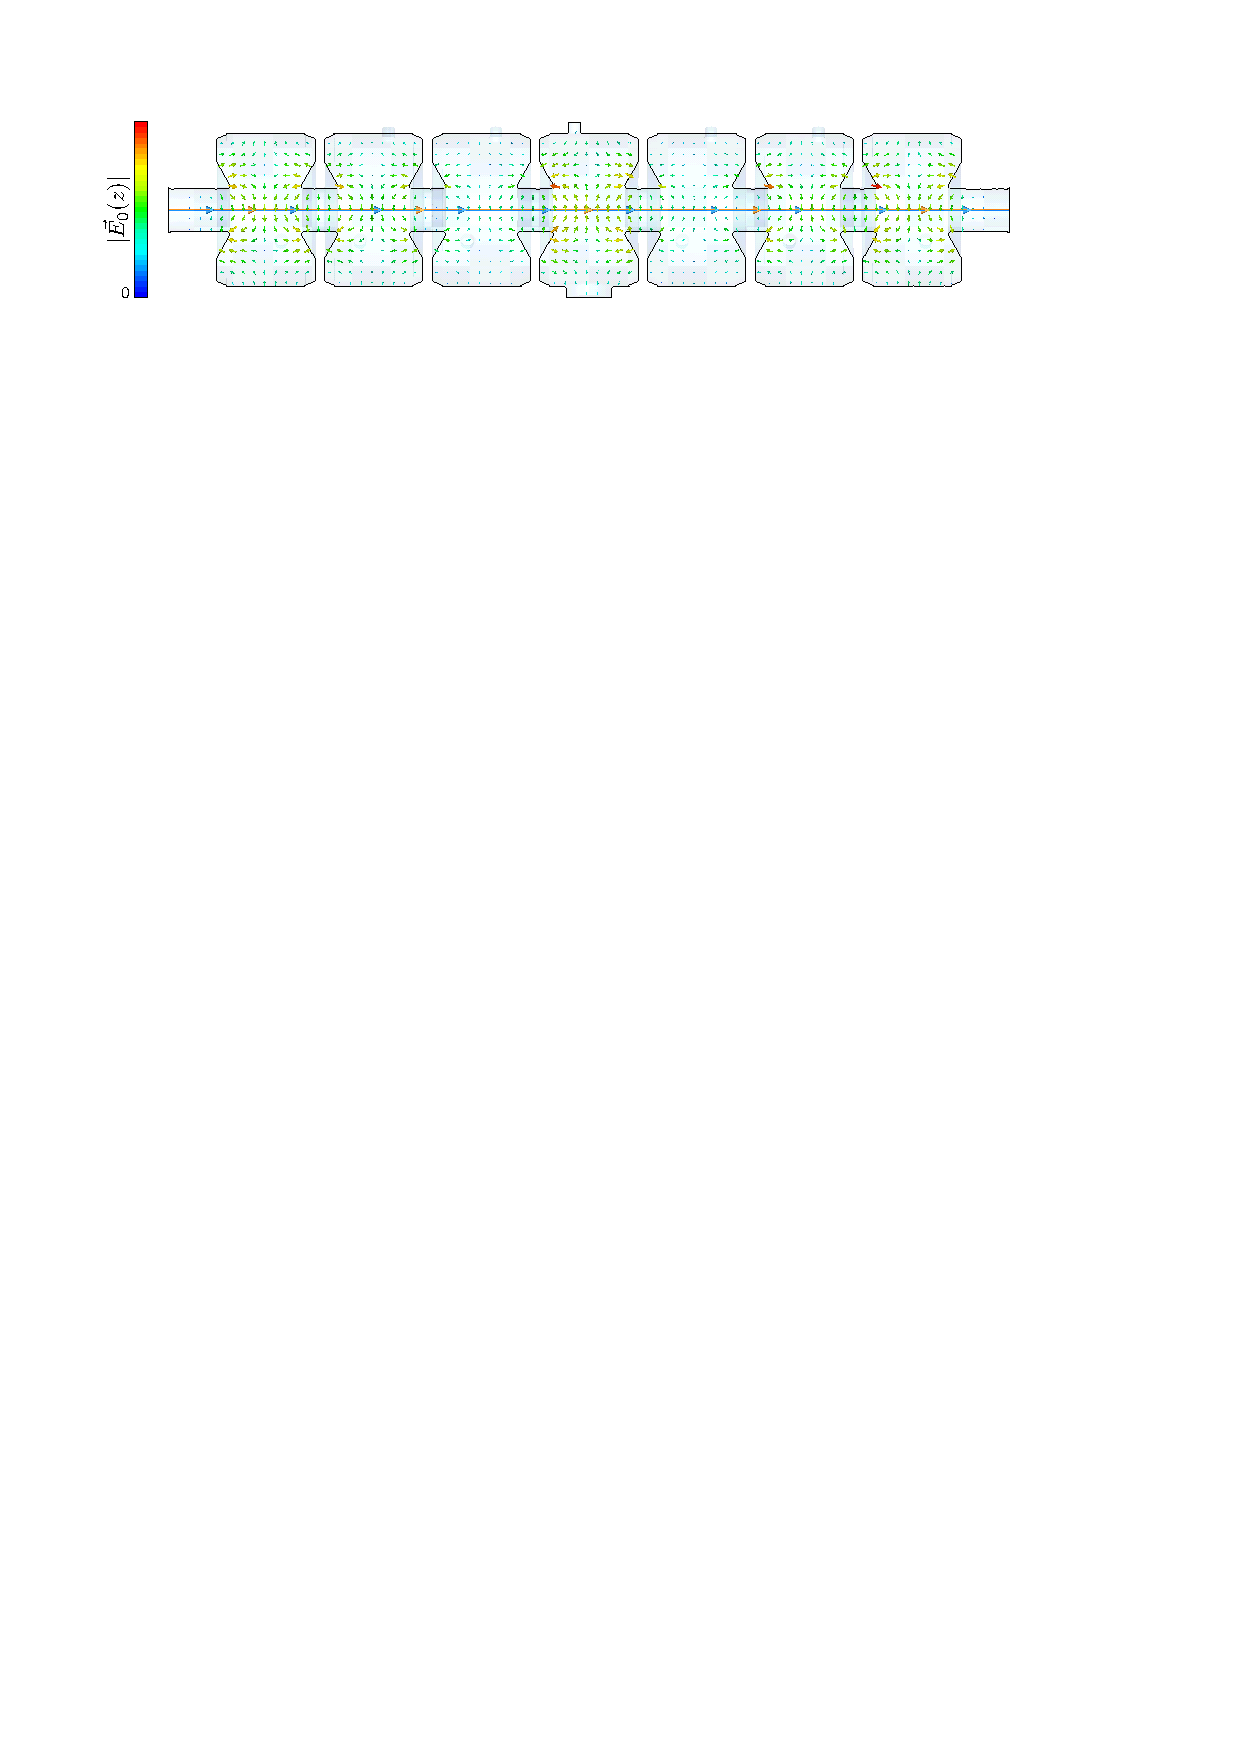
\includegraphics[width=1.0\textwidth]{./figs/TM111-CST/TM111_legende.pdf}
		\caption{Qualitative Darstellung des elektrischen Feldes zu einem festen Zeitpunkt. Gezeigt ist der Querschnitt des Resonator-Modells mit der Strahlenachse in der Schnittebene.}
	\end{subfigure}
	\begin{subfigure}{1\textwidth}
		\centering
		\hspace*{3.5mm}% GNUPLOT: LaTeX picture with Postscript
\begingroup
  \makeatletter
  \providecommand\color[2][]{%
    \GenericError{(gnuplot) \space\space\space\@spaces}{%
      Package color not loaded in conjunction with
      terminal option `colourtext'%
    }{See the gnuplot documentation for explanation.%
    }{Either use 'blacktext' in gnuplot or load the package
      color.sty in LaTeX.}%
    \renewcommand\color[2][]{}%
  }%
  \providecommand\includegraphics[2][]{%
    \GenericError{(gnuplot) \space\space\space\@spaces}{%
      Package graphicx or graphics not loaded%
    }{See the gnuplot documentation for explanation.%
    }{The gnuplot epslatex terminal needs graphicx.sty or graphics.sty.}%
    \renewcommand\includegraphics[2][]{}%
  }%
  \providecommand\rotatebox[2]{#2}%
  \@ifundefined{ifGPcolor}{%
    \newif\ifGPcolor
    \GPcolortrue
  }{}%
  \@ifundefined{ifGPblacktext}{%
    \newif\ifGPblacktext
    \GPblacktexttrue
  }{}%
  % define a \g@addto@macro without @ in the name:
  \let\gplgaddtomacro\g@addto@macro
  % define empty templates for all commands taking text:
  \gdef\gplbacktext{}%
  \gdef\gplfronttext{}%
  \makeatother
  \ifGPblacktext
    % no textcolor at all
    \def\colorrgb#1{}%
    \def\colorgray#1{}%
  \else
    % gray or color?
    \ifGPcolor
      \def\colorrgb#1{\color[rgb]{#1}}%
      \def\colorgray#1{\color[gray]{#1}}%
      \expandafter\def\csname LTw\endcsname{\color{white}}%
      \expandafter\def\csname LTb\endcsname{\color{black}}%
      \expandafter\def\csname LTa\endcsname{\color{black}}%
      \expandafter\def\csname LT0\endcsname{\color[rgb]{1,0,0}}%
      \expandafter\def\csname LT1\endcsname{\color[rgb]{0,1,0}}%
      \expandafter\def\csname LT2\endcsname{\color[rgb]{0,0,1}}%
      \expandafter\def\csname LT3\endcsname{\color[rgb]{1,0,1}}%
      \expandafter\def\csname LT4\endcsname{\color[rgb]{0,1,1}}%
      \expandafter\def\csname LT5\endcsname{\color[rgb]{1,1,0}}%
      \expandafter\def\csname LT6\endcsname{\color[rgb]{0,0,0}}%
      \expandafter\def\csname LT7\endcsname{\color[rgb]{1,0.3,0}}%
      \expandafter\def\csname LT8\endcsname{\color[rgb]{0.5,0.5,0.5}}%
    \else
      % gray
      \def\colorrgb#1{\color{black}}%
      \def\colorgray#1{\color[gray]{#1}}%
      \expandafter\def\csname LTw\endcsname{\color{white}}%
      \expandafter\def\csname LTb\endcsname{\color{black}}%
      \expandafter\def\csname LTa\endcsname{\color{black}}%
      \expandafter\def\csname LT0\endcsname{\color{black}}%
      \expandafter\def\csname LT1\endcsname{\color{black}}%
      \expandafter\def\csname LT2\endcsname{\color{black}}%
      \expandafter\def\csname LT3\endcsname{\color{black}}%
      \expandafter\def\csname LT4\endcsname{\color{black}}%
      \expandafter\def\csname LT5\endcsname{\color{black}}%
      \expandafter\def\csname LT6\endcsname{\color{black}}%
      \expandafter\def\csname LT7\endcsname{\color{black}}%
      \expandafter\def\csname LT8\endcsname{\color{black}}%
    \fi
  \fi
    \setlength{\unitlength}{0.0500bp}%
    \ifx\gptboxheight\undefined%
      \newlength{\gptboxheight}%
      \newlength{\gptboxwidth}%
      \newsavebox{\gptboxtext}%
    \fi%
    \setlength{\fboxrule}{0.5pt}%
    \setlength{\fboxsep}{1pt}%
\begin{picture}(6802.00,2834.00)%
    \gplgaddtomacro\gplbacktext{%
      \csname LTb\endcsname%
      \put(682,704){\makebox(0,0)[r]{\strut{}0}}%
      \put(682,1077){\makebox(0,0)[r]{\strut{}2}}%
      \put(682,1450){\makebox(0,0)[r]{\strut{}4}}%
      \put(682,1823){\makebox(0,0)[r]{\strut{}6}}%
      \put(682,2196){\makebox(0,0)[r]{\strut{}8}}%
      \put(682,2569){\makebox(0,0)[r]{\strut{}10}}%
      \put(814,484){\makebox(0,0){\strut{}0}}%
      \put(2073,484){\makebox(0,0){\strut{}500}}%
      \put(3332,484){\makebox(0,0){\strut{}1000}}%
      \put(4592,484){\makebox(0,0){\strut{}1500}}%
      \put(5851,484){\makebox(0,0){\strut{}2000}}%
    }%
    \gplgaddtomacro\gplfronttext{%
      \csname LTb\endcsname%
      \put(176,1636){\rotatebox{-270}{\makebox(0,0){\strut{}$|\vec{E}_0(z)|$ / willk.\ Einh.}}}%
      \put(3609,154){\makebox(0,0){\strut{}$z$ / \si{mm}}}%
    }%
    \gplbacktext
    \put(0,0){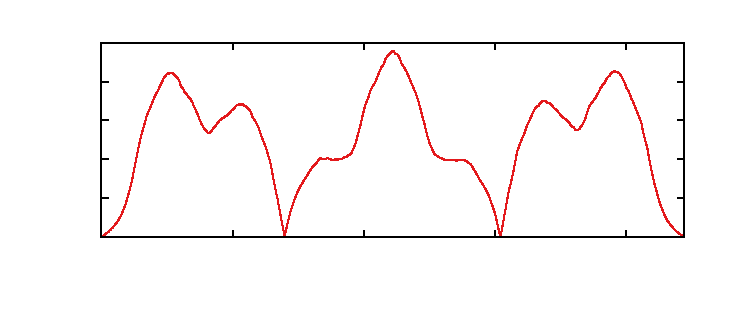
\includegraphics{./plots/tm111_abs_sim}}%
    \gplfronttext
  \end{picture}%
\endgroup

		\caption{Amplitude des elektrischen Feldes in Abhängigkeit der Position auf der Strahlenachse.}
	\end{subfigure}
	\caption[Simulation der $\mathrm{TM}_{111}$-Eigenmode des PETRA-Resonators durch CST-MWS]{Simulation der vermessenen $\mathrm{TM}_{111}$-Eigenmode durch CST-MWS.}
	\label{fig:cst_sim_tm111}
\end{figure}
Ein wichtiges Merkmal ist das Verschwinden des elektrischen Feldes zwischen Zellen mit einem Phasensprung des elektrischen Feldes von $\pi$.
Dies ist zwischen der zweiten und dritten Zelle in Abbildung \ref{fig:cst_sim_tm111} zu beobachten und kann zur eindeutigen Identifikation der meisten Resonatormoden und deren Phasenbeziehung genutzt werden.

Für zwei der vermessenen Moden ist keine eindeutige Bestimmung der Phasenbeziehung zu vollziehen, da diese keinen Eigenmoden der Simulation durch CST-MWS zugeordnet werden können.
Außerdem ist eine Festlegung der Phasenbeziehung durch das zuvor erwähnte Merkmal nicht möglich, da die betroffenen Moden eine verschwindende elektrische Feldamplitude in den mittleren Zellen aufweisen (vgl.\ Abb.\ \ref{fig:tm021_1458} f.).
Daher wird für diese Moden die Phasenbeziehung so gewählt, dass der Fall maximaler effektiver Shuntimpedanz eintritt.

Für Moden höherer Ordnung können gemäß Abschnitt \ref{sec:em_felder_in_resonatoren} auch $\pi$-Phasensprünge innerhalb einer Zelle stattfinden (z.\ B.\ bei den $\mathrm{TM}_{021}$-Moden), welche ebenfalls bei der Auswertung beachtet werden müssen.

Die restliche Auswertung folgt analog zu Abschnitt \ref{sec:tm010_messung} und die Ergebnisse wurden in Tabelle~\ref{tab:shuntimpedanzen_hom} dargestellt.
Die Darstellungen der elektrischen Felder wurde in Abschnitt~\ref{app:hom_felder} zusammengefasst.
\begin{table}[htb]
	\centering
	\begin{tabular}{
		c
		c
		S[table-format=4.2]
		S[table-format=5.0(3), table-align-uncertainty = true]
		S[table-format=1.3(3), table-align-uncertainty = true]
		S[table-format=0.3(1), table-align-uncertainty = true]
		S[table-format=3.2(2), table-align-uncertainty = true]
		}
	\toprule
	\multicolumn{2}{c}{Mode} & {$\nu_0$ / \si{MHz}} & {$Q_0$} & {$R_\mathrm{S}$ / \si{\mega\ohm}} & {$\Lambda$} & {$R_\mathrm{S}^\mathrm{eff}$ / \si{\kilo\ohm}} \\
	\midrule
	$\mathrm{TE}_{111}$ & trans. & 702.70 & 11162+-18 & 3.89+-0.14 & 0.289+-0.002 & 326+-11 \\[0.25em]
	$\mathrm{TM}_{011}$ & long. & 730.45 & 13927+-39 & 3.28+-0.12 & 0.118+-0.003 & 45.8+-1.6 \\[0.25em]
	$\mathrm{TM}_{111}$ & trans. & 1047.23 & 28528+-174 & 8.14+-0.29 & 0.017+-0.001 & 2.34+-0.15 \\[0.25em]
	---\textsuperscript{\textasteriskcentered} & long. & 1375.79 & 59762+-416 & 9.47+-0.34 & 0.019+-0.002 & 3.40+-0.40 \\[0.25em]
	$\mathrm{TM}_{021}$\textsuperscript{\textdagger} & long. & 1458.30 & 7552+-51 & 0.566+-0.020 & 0.182+-0.004 & 18.8+-0.7 \\[0.25em]
	$\mathrm{TM}_{021}$\textsuperscript{\textdagger} & long. & 1460.34 & 16043+-63 & 0.729+-0.026 & 0.266+-0.004 & 51.7+-1.8 \\[0.25em]
	$\mathrm{TM}_{021}$ & long. & 1464.96 & 25279+-172 & 2.60+-0.10 & 0.100+-0.002 & 26.1+-1.0 \\[0.25em]
	$\mathrm{TM}_{021}$ & long. & 1465.83 & 15028+-92 & 2.52+-0.09 & 0.269+-0.001 & 183.0+-6.4 \\
	\midrule
	\multicolumn{7}{l}{
		\small{\textsuperscript{\textasteriskcentered}: Nicht Klassifizierbar nach zylindrischen Hohlräumen}
	}\\
	\multicolumn{7}{l}{
		\small{\textsuperscript{\textdagger}: Für Phasenbeziehung wurde worst-case angenommen}
	}\\
	\bottomrule
\end{tabular}

	\caption[Longitudinale/Transversale Shuntimpedanzen der Moden höherer Ordnung von PETRA-III]{Longitudinale/Transversale Shuntimpedanzen der vermessenen Moden höherer Ordnung von PETRA-III. Die Resonanzfrequenz $\nu_0$ wurde gemäß Abschnitt \ref{sec:vorbereitung_resonator} auf die Frequenz des evakuierten Resonators umgerechnet.}
	\label{tab:shuntimpedanzen_hom}
\end{table}


\subsection{Interpretation der Ergebnisse}
Bevor eine Diskussion der resultierenden Shuntimpedanzen erfolgt, sollen die gemessenen Verteilungen des elektrischen Feldes erörtert werden.
Einerseits fällt bei Betrachtung der Feldverteilungen in Abschnitt \ref{app:hom_felder} auf, dass Sprünge des effektiven elektrischen Feldes auftreten.
Diese entstehen an Stellen, an denen das elektrische Feld einen Phasensprung vollzieht und ist auf die begrenzte Ortsauflösung durch die Ausdehnung des verwendeten Störkörpers zurückzuführen.
%Dies ist der Fall, da an solchen Stellen ein Knoten der elektrischen Feldstärke vorliegt, welcher bei der Störkörpermessung nicht als solcher erscheint, da aufgrund der Ausdehnung des Störkörpers eine Frequenzverschiebung durch die umliegenden Stellen nicht-verschwindender Amplitude zu einer Frequenzverschiebung führen.
Bei der Bestimmung der Shuntimpedanzen durch Integration stellen diese Sprungstellen jedoch keinen signifikanten Einfluss dar und können vernachlässigt werden.
Mit der Verwendung eines kleineren Störkörpers wäre dennoch eine Möglichkeit gegeben, diese Sprünge zu vermindern, was jedoch mit einer Abnahme der Frequenzverschiebung durch die Störung der Resonatormoden zusammenhängen würde.
Insbesondere bei den Moden höherer Ordnung, die im Vergleich zur Fundamentalmode kleine Feldstärken aufweisen, kann dies eine Temperaturstabilisierung von Resonator und VNA erfordern und wurde daher nicht ausgenutzt.

Ferner führt die über den Messbereich konstante Frequenzauflösung des VNA und die Proportionalität
\begin{align}
\frac{|\ve_0|}{\sqrt{P_\mathrm{V}}} \propto \sqrt{\Delta \omega}
\end{align}
aus Gl.\ \eqref{eq:skm_e_feld_normiert} zu einer Abnahme der Auflösung, mit der die Amplitude des elektrischen Feldes gemessen werden kann, bei kleinen Amplituden des Feldes.
Dies führt dazu, dass Feldamplituden, die unter die Auflösungsgrenze fallen, nicht von einem verschwindenden elektrischen Feld zu unterscheiden sind.
Dadurch kann an manche Moden mit scheinbar verschwindendem elektrischen Feld (und damit auch magnetischem Feld) in der mittleren Resonatorzelle (vgl.\ Abb.\ \ref{fig:tm021_1458} ff.) eine Kopplung stattfinden.

Generell zeigen die meisten vermessenen Moden eine Shuntimpedanz~$R_\mathrm{S}^\mathrm{eff}$ von einigen \si{\mega\ohm}.
Jedoch führen die kleinen Laufzeitfaktoren~$\Lambda$ gemäß Gl.\ \eqref{eq:eff_shuntimpedanz} zu einer Reduzierung der effektiven Shuntimpedanz um den Faktor $\Lambda^2$.
Dies resultiert darin, dass die effektiven Shuntimpedanzen Werte in der Größenordnung von einigen \si{\kilo\ohm} annehmen.
Die größte effektive Shuntimpedanz zeigt dabei die $\mathrm{TE_{111}}$-Mode mit $\SI{326 +- 11}{\kilo\ohm}$ (transversal).
Der Vergleich mit der effektiven Shuntimpedanz der Fundamentalmode von etwa \SI{25}{\mega\ohm} zeigt bereits, dass der parasitäre Einfluss dieser Mode gegenüber der Fundamentalmode klein ist.
Darüber hinaus zeigt die Mode mit der Resonanzfrequenz \SI{1465.83}{MHz} die größte effektive Shuntimpedanz der $\mathrm{TM}_{021}$-Moden.
Diese liegt bei \SI{183.0 +- 6.4}{\kilo\ohm} und fällt damit ebenfalls zwei Größenordnungen unter die effektive Shuntimpedanz der Fundamentalmode.

Abschließend ist zu bemerken, dass entgegen der Erwartung keine der vermessenen Moden höherer Ordnung effektive Shuntimpedanzen in der Größenordnung der Fundamentalmode aufweist.
Dennoch ist anzumerken, dass die Untersuchung dieser Moden keineswegs umfassend war, da eine unendliche Anzahl von Moden höherer Ordnung existieren.
Bei einer weitergehenden Analyse ist eine Simulation des Impedanzspektrums (z.\ B.\ durch \textit{CST Particle Studio\textsuperscript{\textregistered}}) unter Verwendung eines detaillierteren Modells des Resonators zweckmäßig, da dadurch eine bessere Identifizierung der kritischen Moden vollzogen werden kann.
Außerdem kann dadurch eine Untersuchung des Einflusses von Moden höherer Ordnung auf Multi-Bunch-Instabilitäten an ELSA durchgeführt werden.
